\section{Quality Attributes Scenarios (QAS)}
System quality attributes have been of interest to the software community at least since the 1970s. There are a variety of published taxonomies and definitions, and many of them have their own research and practitioner communities. From an architect's perspective, there are three problems with previous discussions of system quality attributes:

\begin{itemize}
  \item The definitions provided for an attribute are not operational. It is meaningless to say that a system will be modifiable. Every system is modifiable with respect to one set of changes and not modifiable with respect to another. The other attributes are similar.
  \item A focus of discussion is often on which quality a particular aspect belongs to. Is a system failure an aspect of availability, an aspect of security, or an aspect of usability? All three attribute communities would claim ownership of a system failure.
  \item Each attribute community has developed its own vocabulary. The performance community has "events" arriving at a system, the security community has "attacks" arriving at a system, the availability community has "failures" of a system, and the usability community has "user input." All of these may actually refer to the same occurrence, but are described using different terms.
\end{itemize}

A solution to the first two of these problems (nonoperational definitions and overlapping attribute concerns) is to use Quality Attribute Scenarios as a means of characterizing quality attributes. A solution to the third problem is to provide a brief discussion of each attribute-concentrating on its underlying concerns-to illustrate the concepts that are fundamental to that attribute community.

\begin{figure}[H]
  \centering
  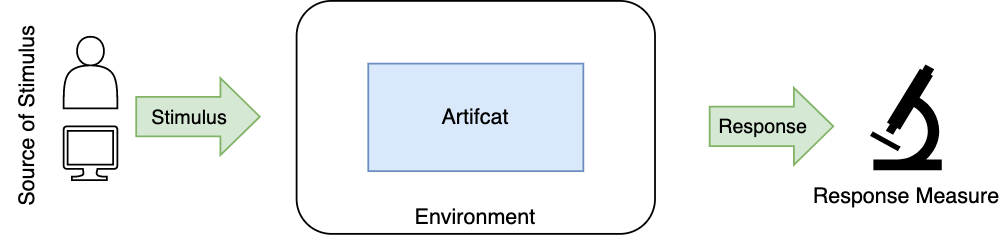
\includegraphics[width=0.8\textwidth]{qualityattributescenario.png}
  \caption{Quality Attribute Scenario Visualization}
\end{figure}

\begin{figure}[H]
  \center
  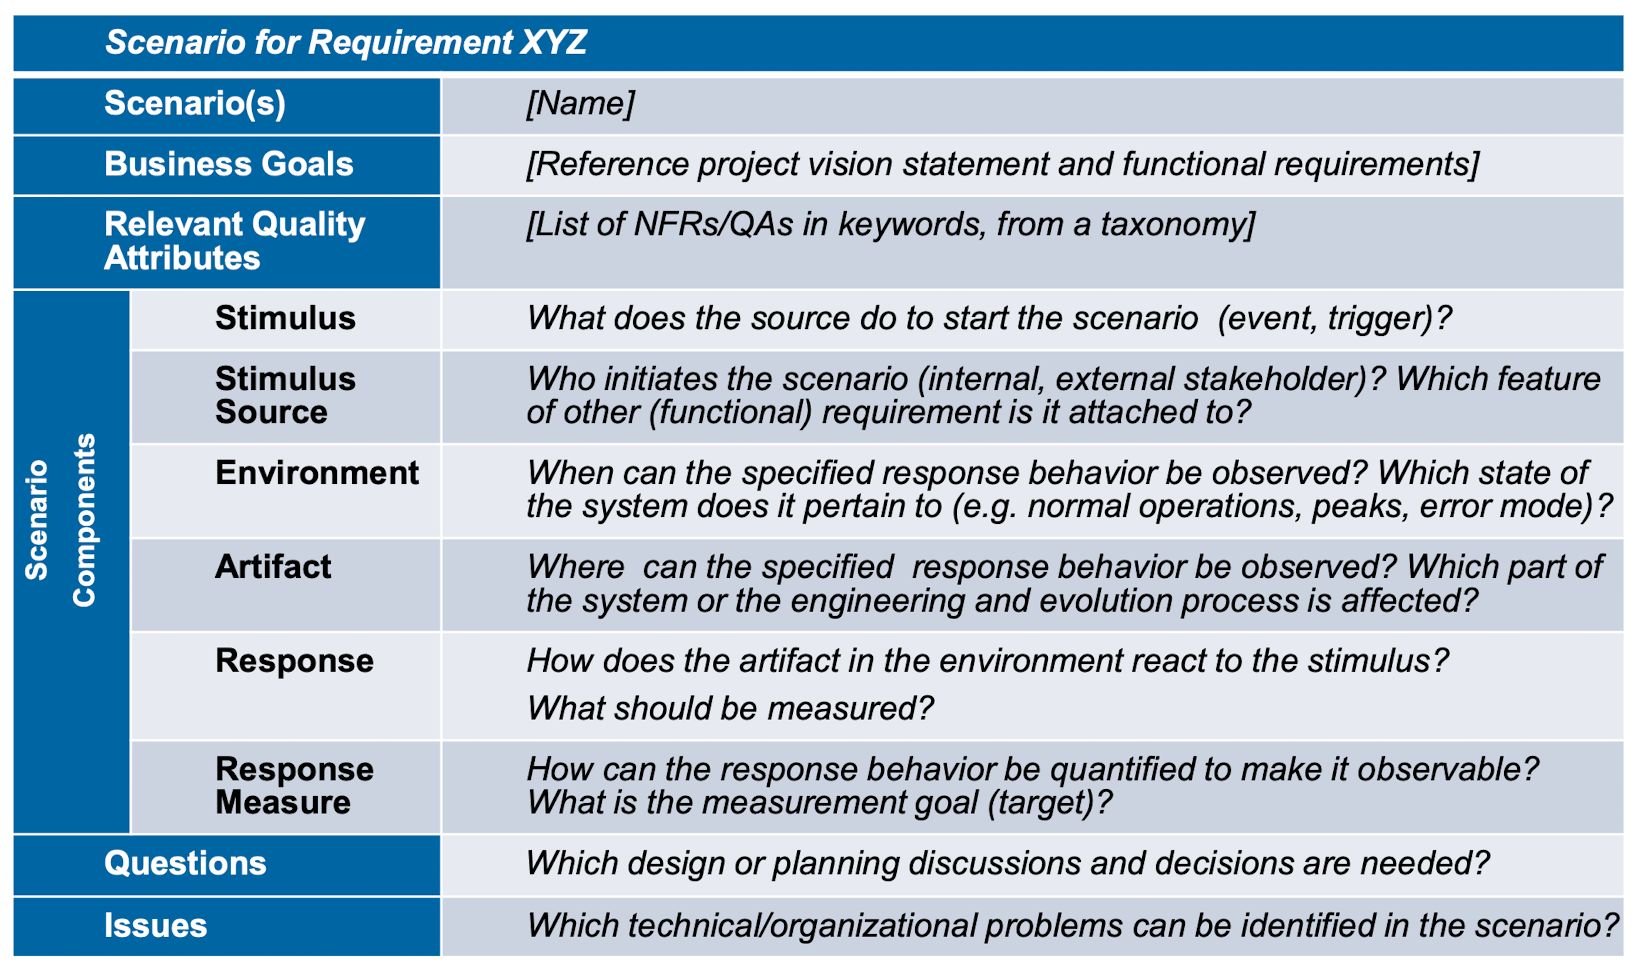
\includegraphics[width=0.8\textwidth]{QAS}
  \caption{Quality Attribute Scenario (QAS) Template}
\end{figure}

\subsection{Landing Zone}
At first glance a landing zone seems nothing more than a glorified table. Each row in the landing zone represents a measurable requirement. Each requirement has a range of acceptable values labeled Minimum, Target, and Outstanding. The goal is to have each requirement within this range at the end of development. This can be used to defined a better Response Measure in the QAS.

The Landing Zone allows for some flexibility in the development of an application and tolerance in the acceptance values.

\begin{figure}[H]
  \center
  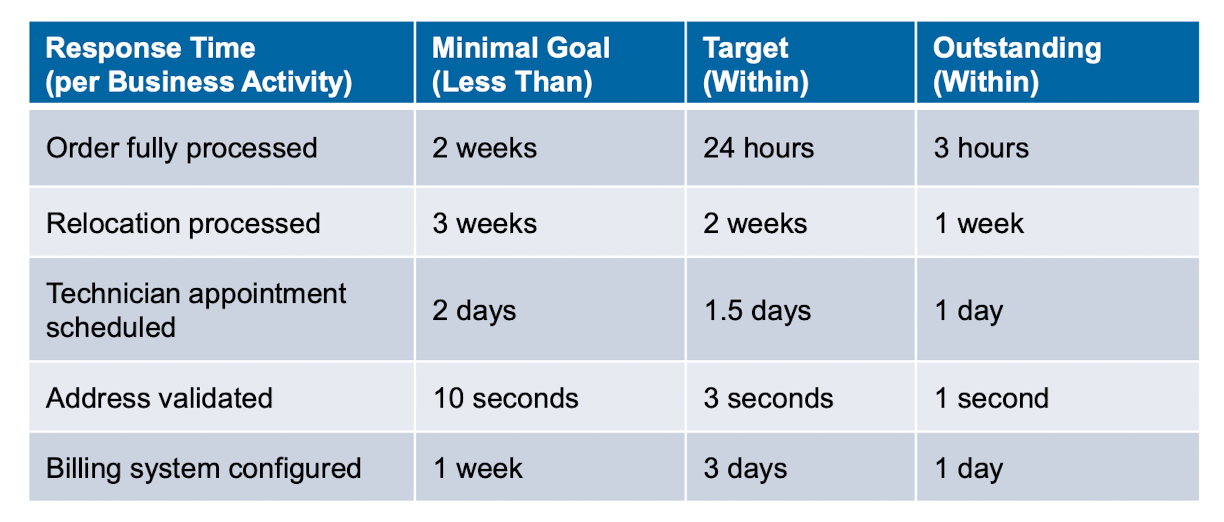
\includegraphics[width=0.75\textwidth]{landingzone}
  \caption{Landing Zone}
\end{figure}

\subsection{Quality Utility Trees}
The Quality Utility Tree is a structure to visualize QAS, which are the leaves of the tree which are priorized py value and risk (V, R) which is shown in Figure \ref{fig:qualityutilitytree}.

\begin{figure}[H]
  \center
  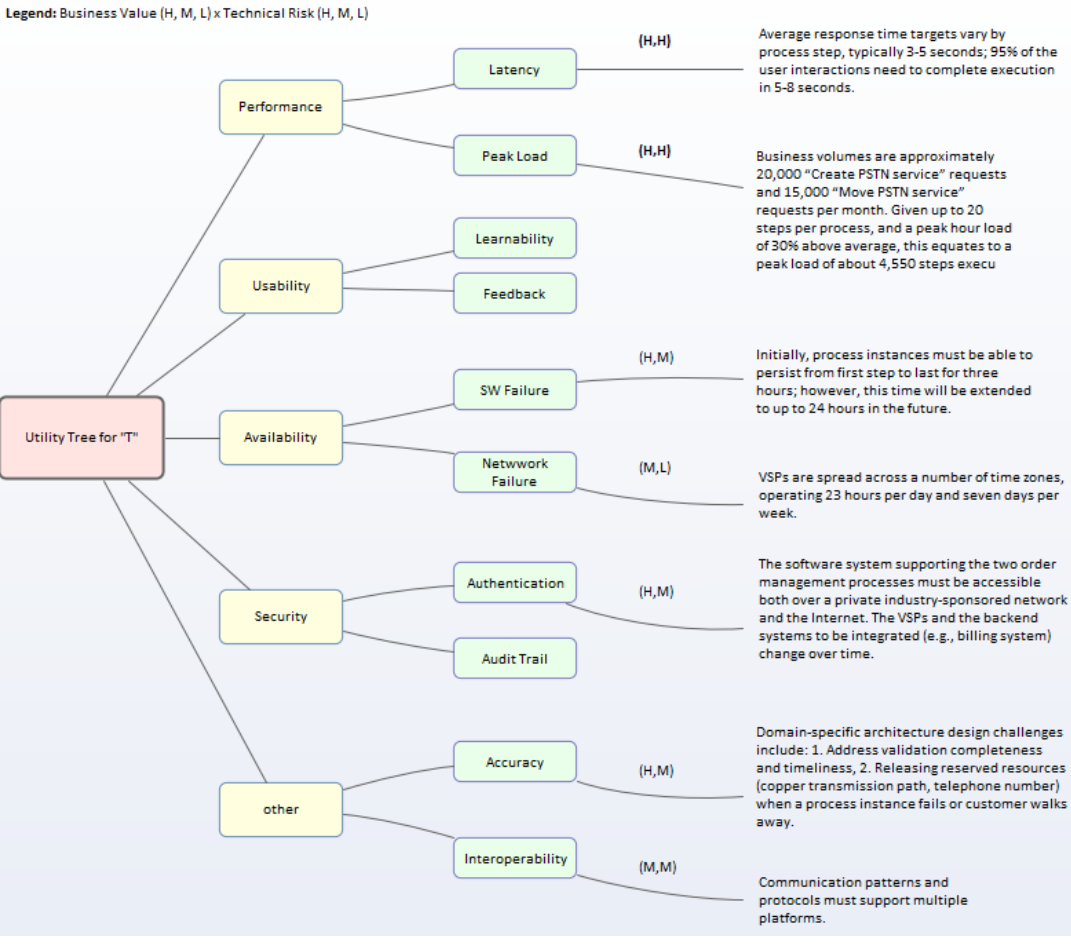
\includegraphics[width=0.9\textwidth]{qualityutilitytrees.png}
  \caption{Quality Utility Tree}
  \label{fig:qualityutilitytree}
\end{figure}

\subsection{Twin Peaks Model}
The importance of interleaving the tasks of eliciting and specifying requirements with that of designing a software solution has long been recognized. The traditional waterfall process produces artificially frozen requirements that often lead to suboptimal architectural solutions, which themselves are often inflexible to future change. Incremental development processes partially address this problem by allowing developers to evaluate repeatedly changing project risks in order to embrace new requirements and to address changing project constraints. The twin peaks model provides an even finer-grained iteration across requirements and architecture that acknowledges the need to develop software architectures that are stable, yet adaptable, in the presence of changing requirements.

As shown in Figure \ref{fig:twinpeakmodel}, the twin peaks model focuses on the co-development of requirements and architecture. Through a series of iterations, the model captures the progression from general to detailed understanding and expression of both requirements and design. Although the schematic of the twin peaks model shows the process initiated on the requirements peak, projects involving modifications to existing systems could be initiated equally well at the architecture peak.

\begin{figure}[h!]
  \center
  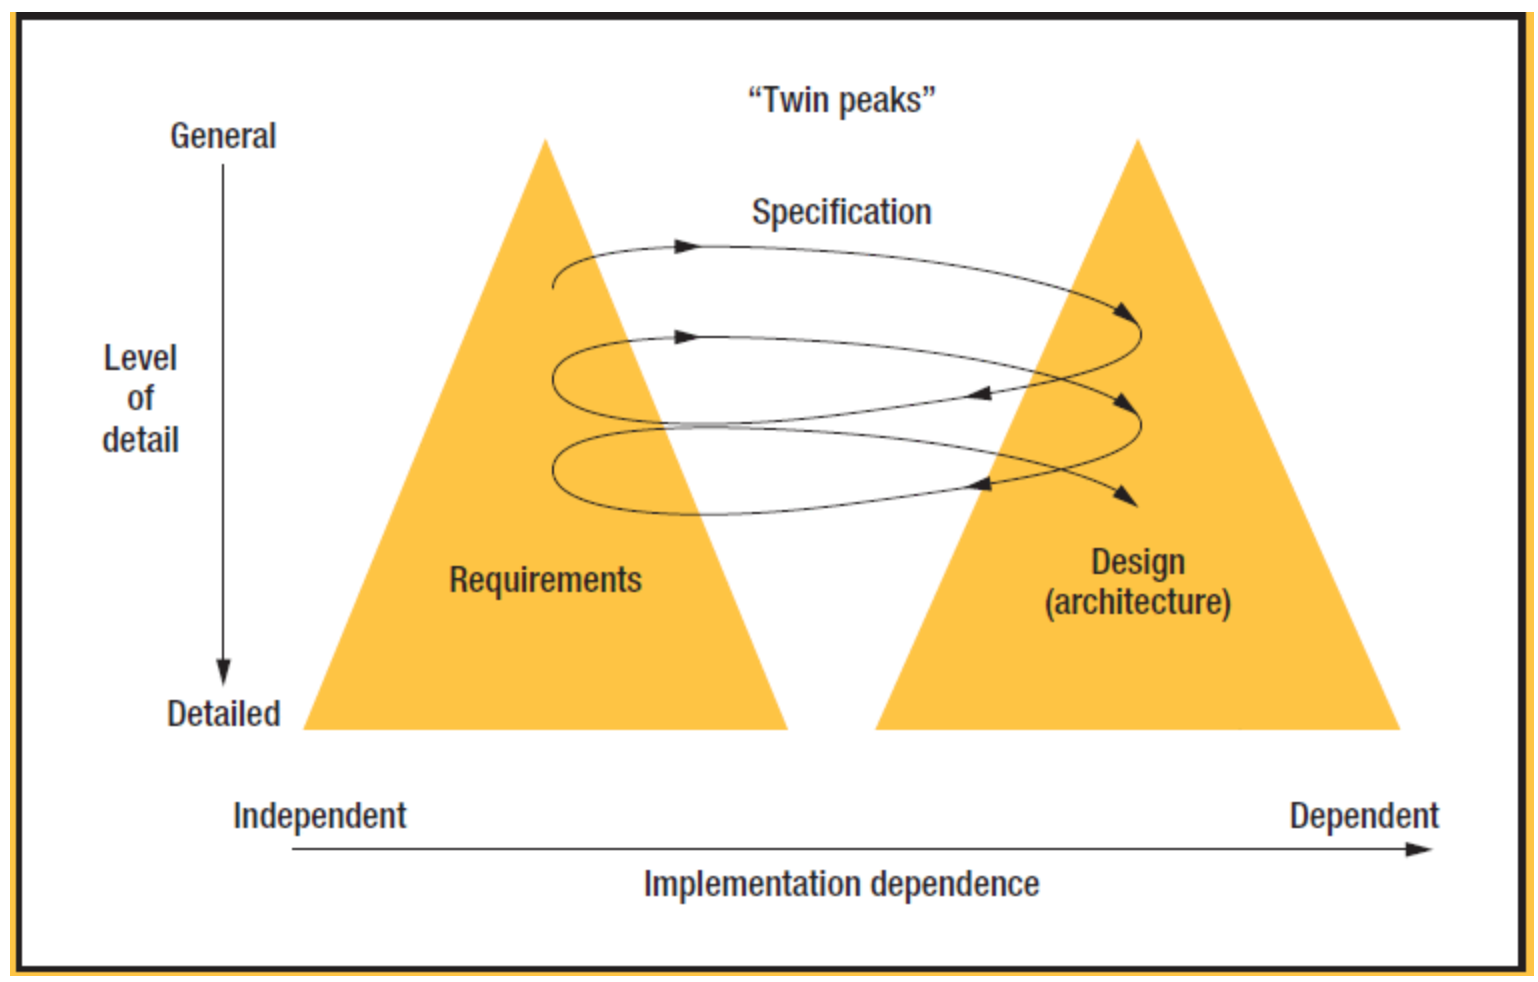
\includegraphics[width=0.65\textwidth]{twinpeakmodel}
  \caption{IEEE Twin Peak Model}
  \label{fig:twinpeakmodel}
\end{figure}

\section{C4 Model for Architecture Visualization}
The C4 model considers the static structures of a software system in terms of containers (applications, data stores, microservices, etc.), components, and code. It also considers the people who use the software systems that we build. The C4 model has predefined modelling entities defined in Figure \ref{fig:c4modelnotation}. The following section does display multiple sample visualizations and there are still further diagrams such as: System Landscape, Dynamic, Deployment diagram. Additionaly the follwing \href{https://www.youtube.com/watch?v=x2-rSnhpw0g}{talk} by the creator of the C4 Model, Simon Brown, gives a good overview of it.

\begin{figure}[H]
  \center
  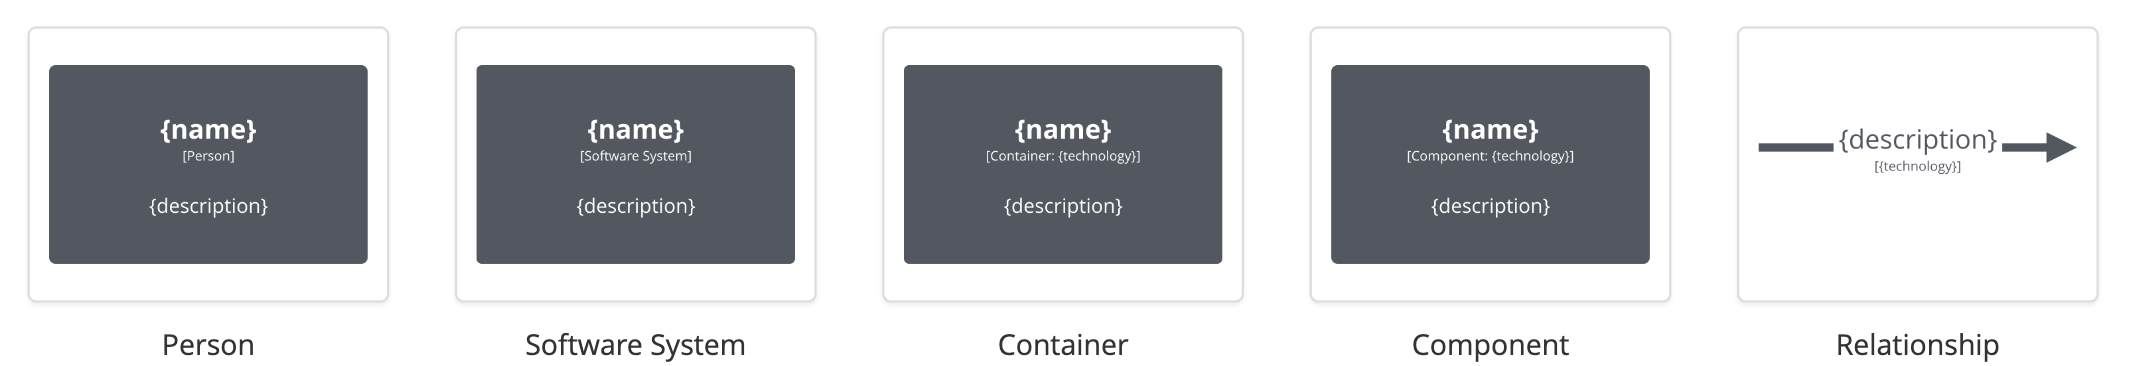
\includegraphics[width=\textwidth]{c4modelnotation}
  \caption{C4 Model Notation}
  \label{fig:c4modelnotation}
\end{figure}

\subsection{Level 1: System Context Diagram}
A system context diagram, shows the software system you are building and how it fits into the world in terms of the people who use it and the other software systems it interacts with.

\begin{figure}[H]
  \center
  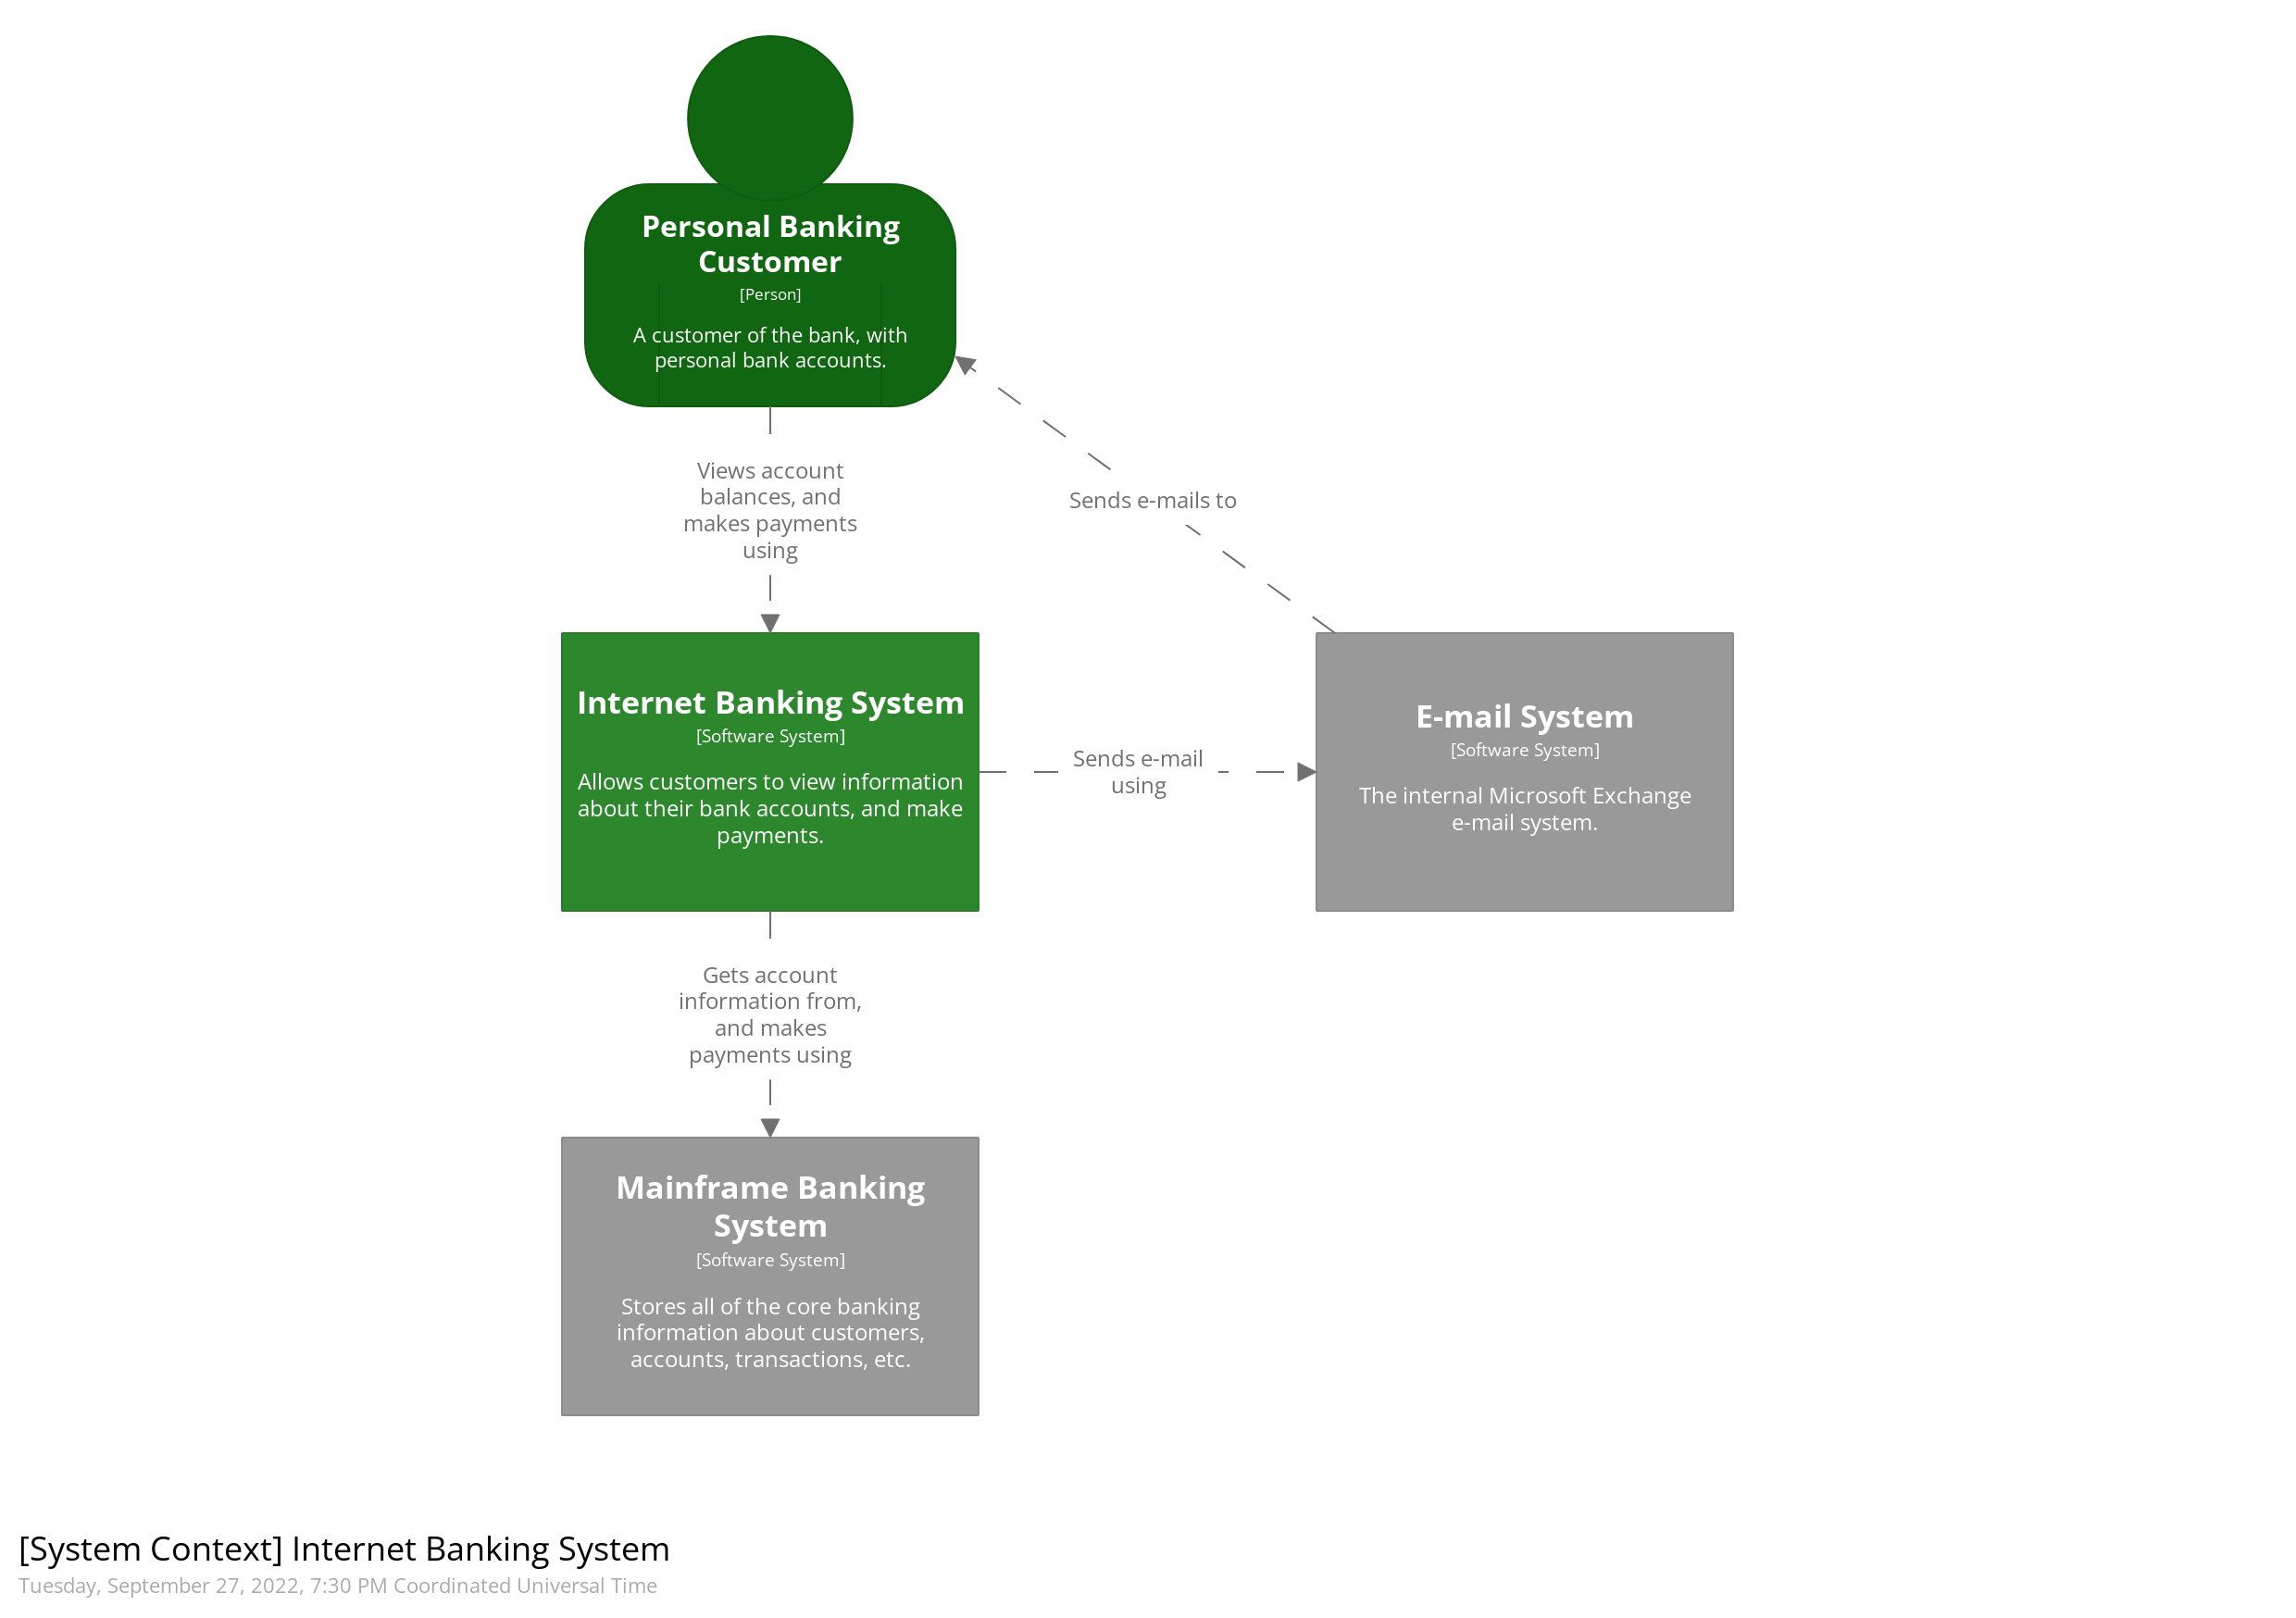
\includegraphics[width=0.75\textwidth]{c4context}
  \caption{C4 Context Diagram}
\end{figure}

\pagebreak

\subsection{Level 2: Container Diagram}
A container diagram, zooms into the software system, and shows the containers (applications, data stores, microservices, etc.) that make up that software system. Technology decisions are also a key part of this diagram.

\begin{figure}[H]
  \center
  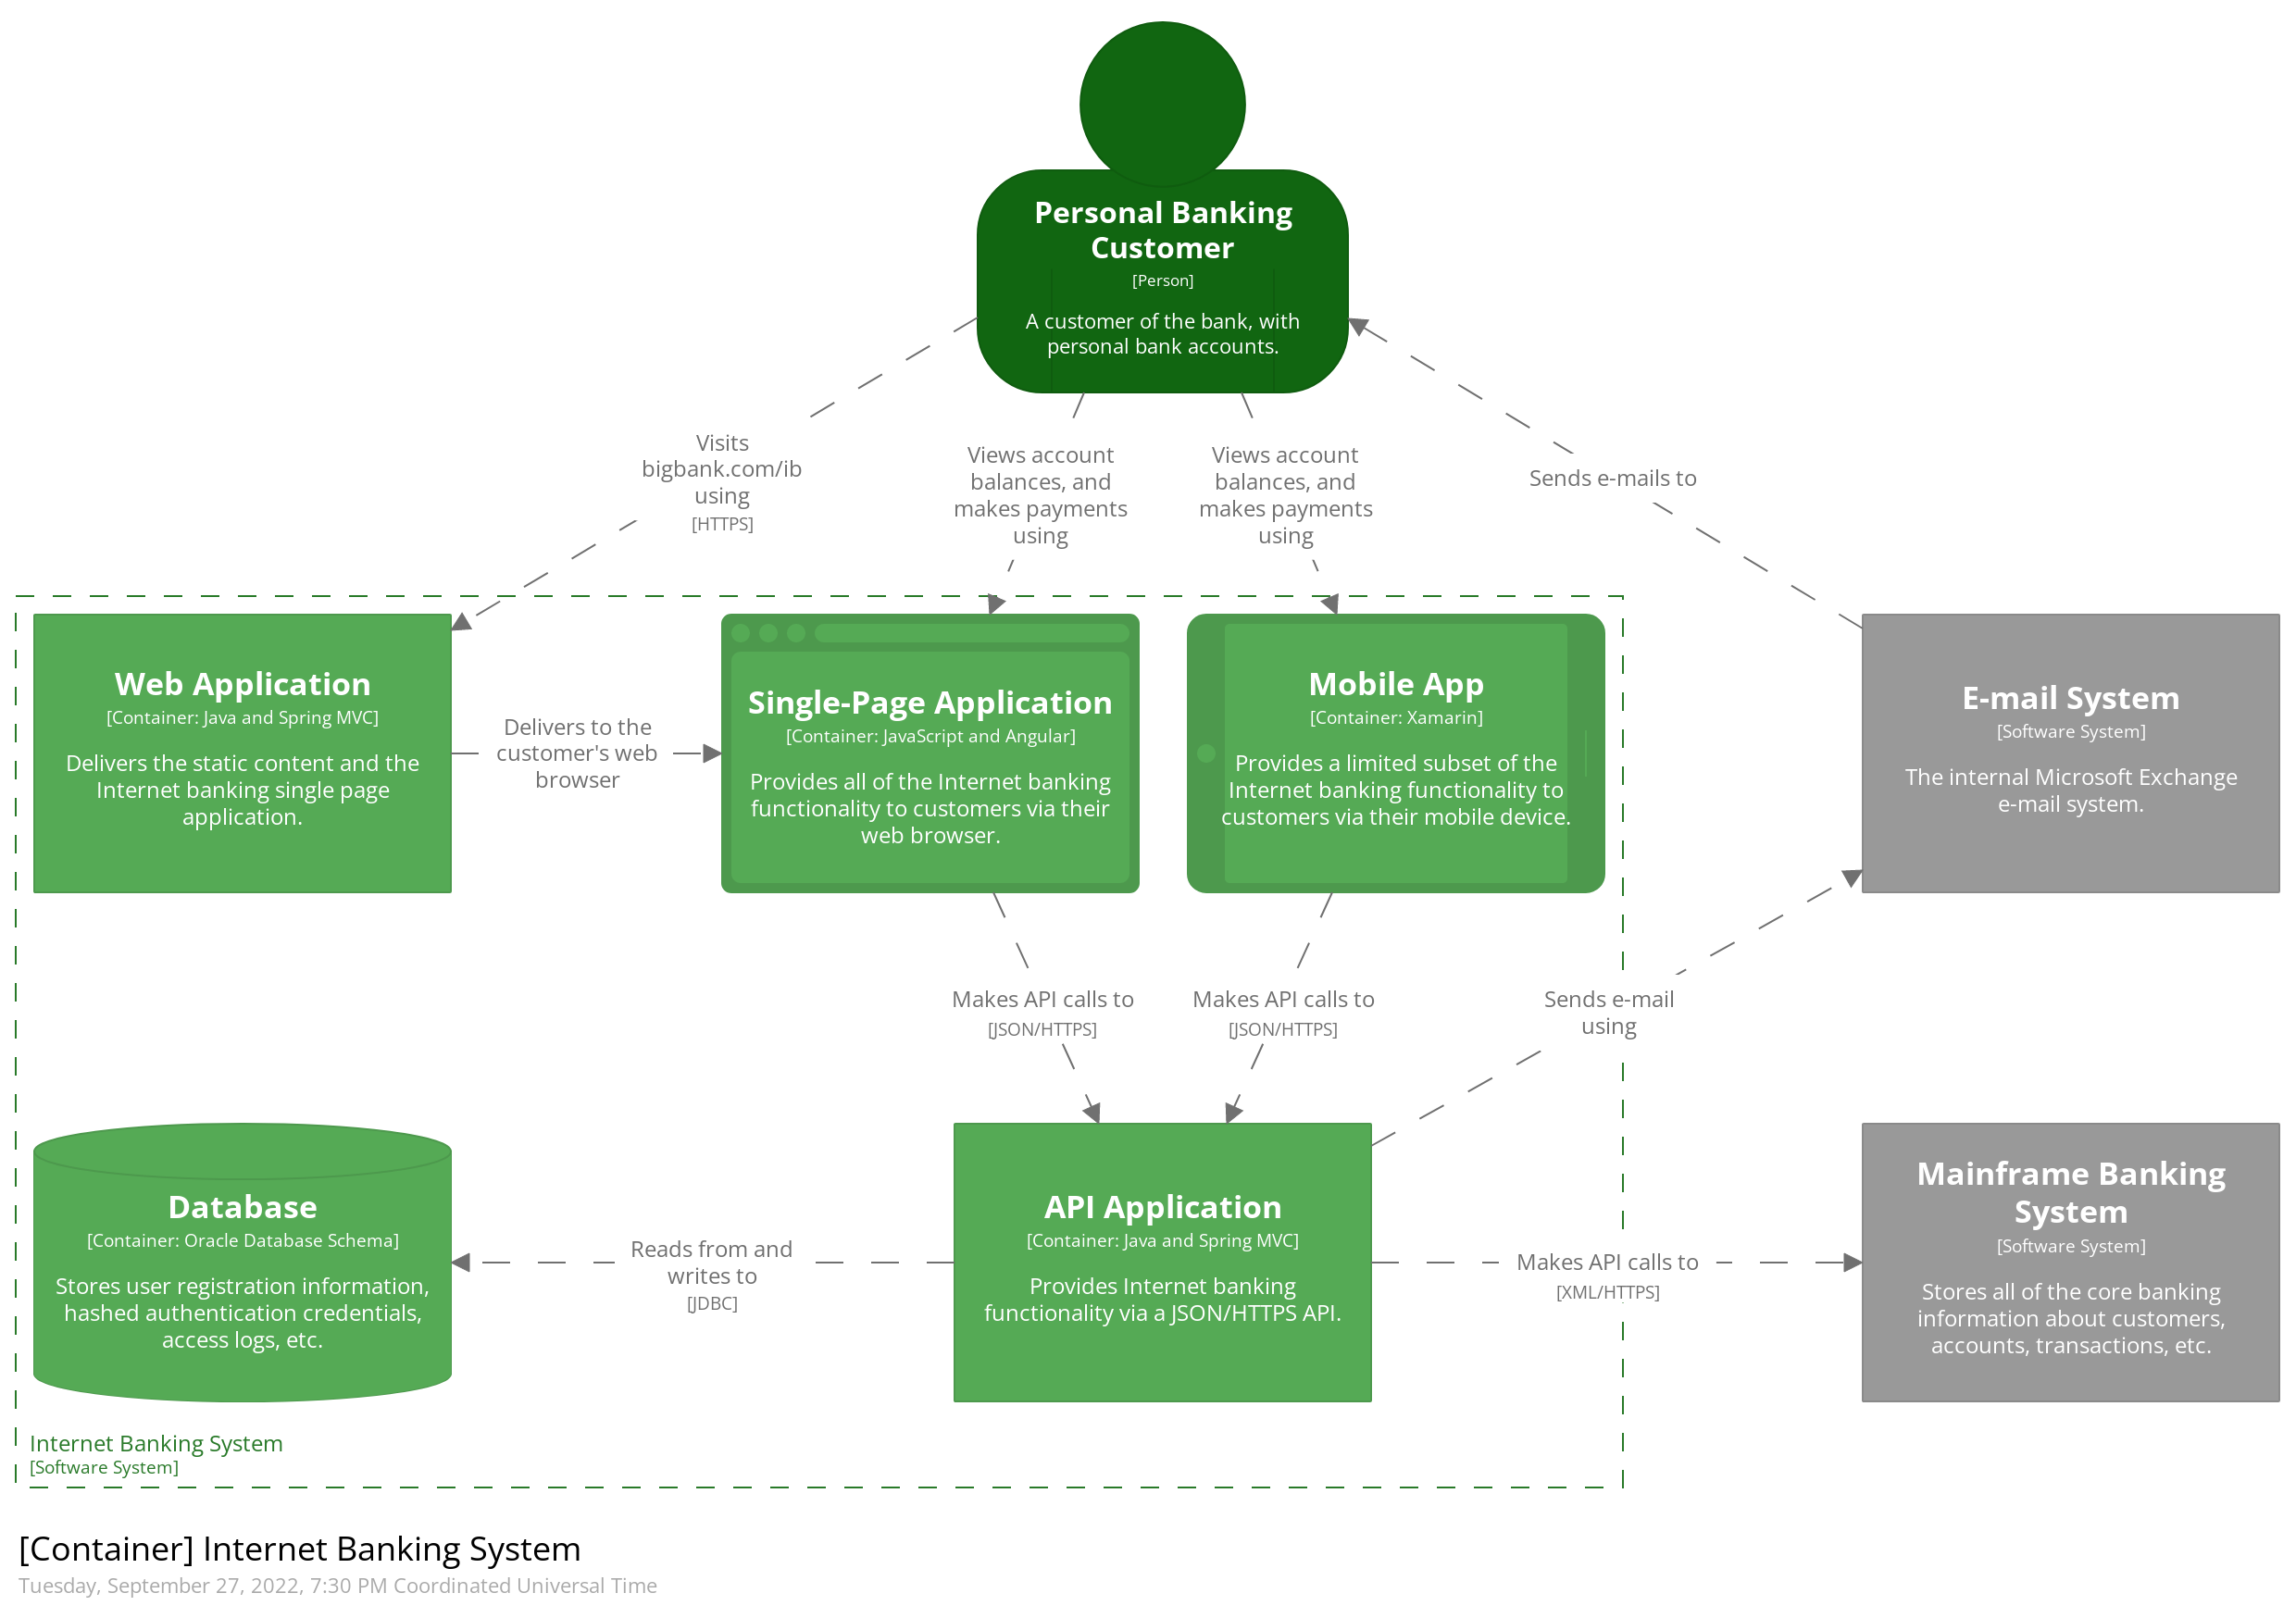
\includegraphics[width=0.75\textwidth]{c4container}
  \caption{C4 Container Diagram}
\end{figure}

\subsection{Level 3: Component Diagram}
A component diagram, zooms into an individual container to show the components inside it. These components should map to real abstractions (e.g., a grouping of code) in your codebase.

\begin{figure}[H]
  \center
  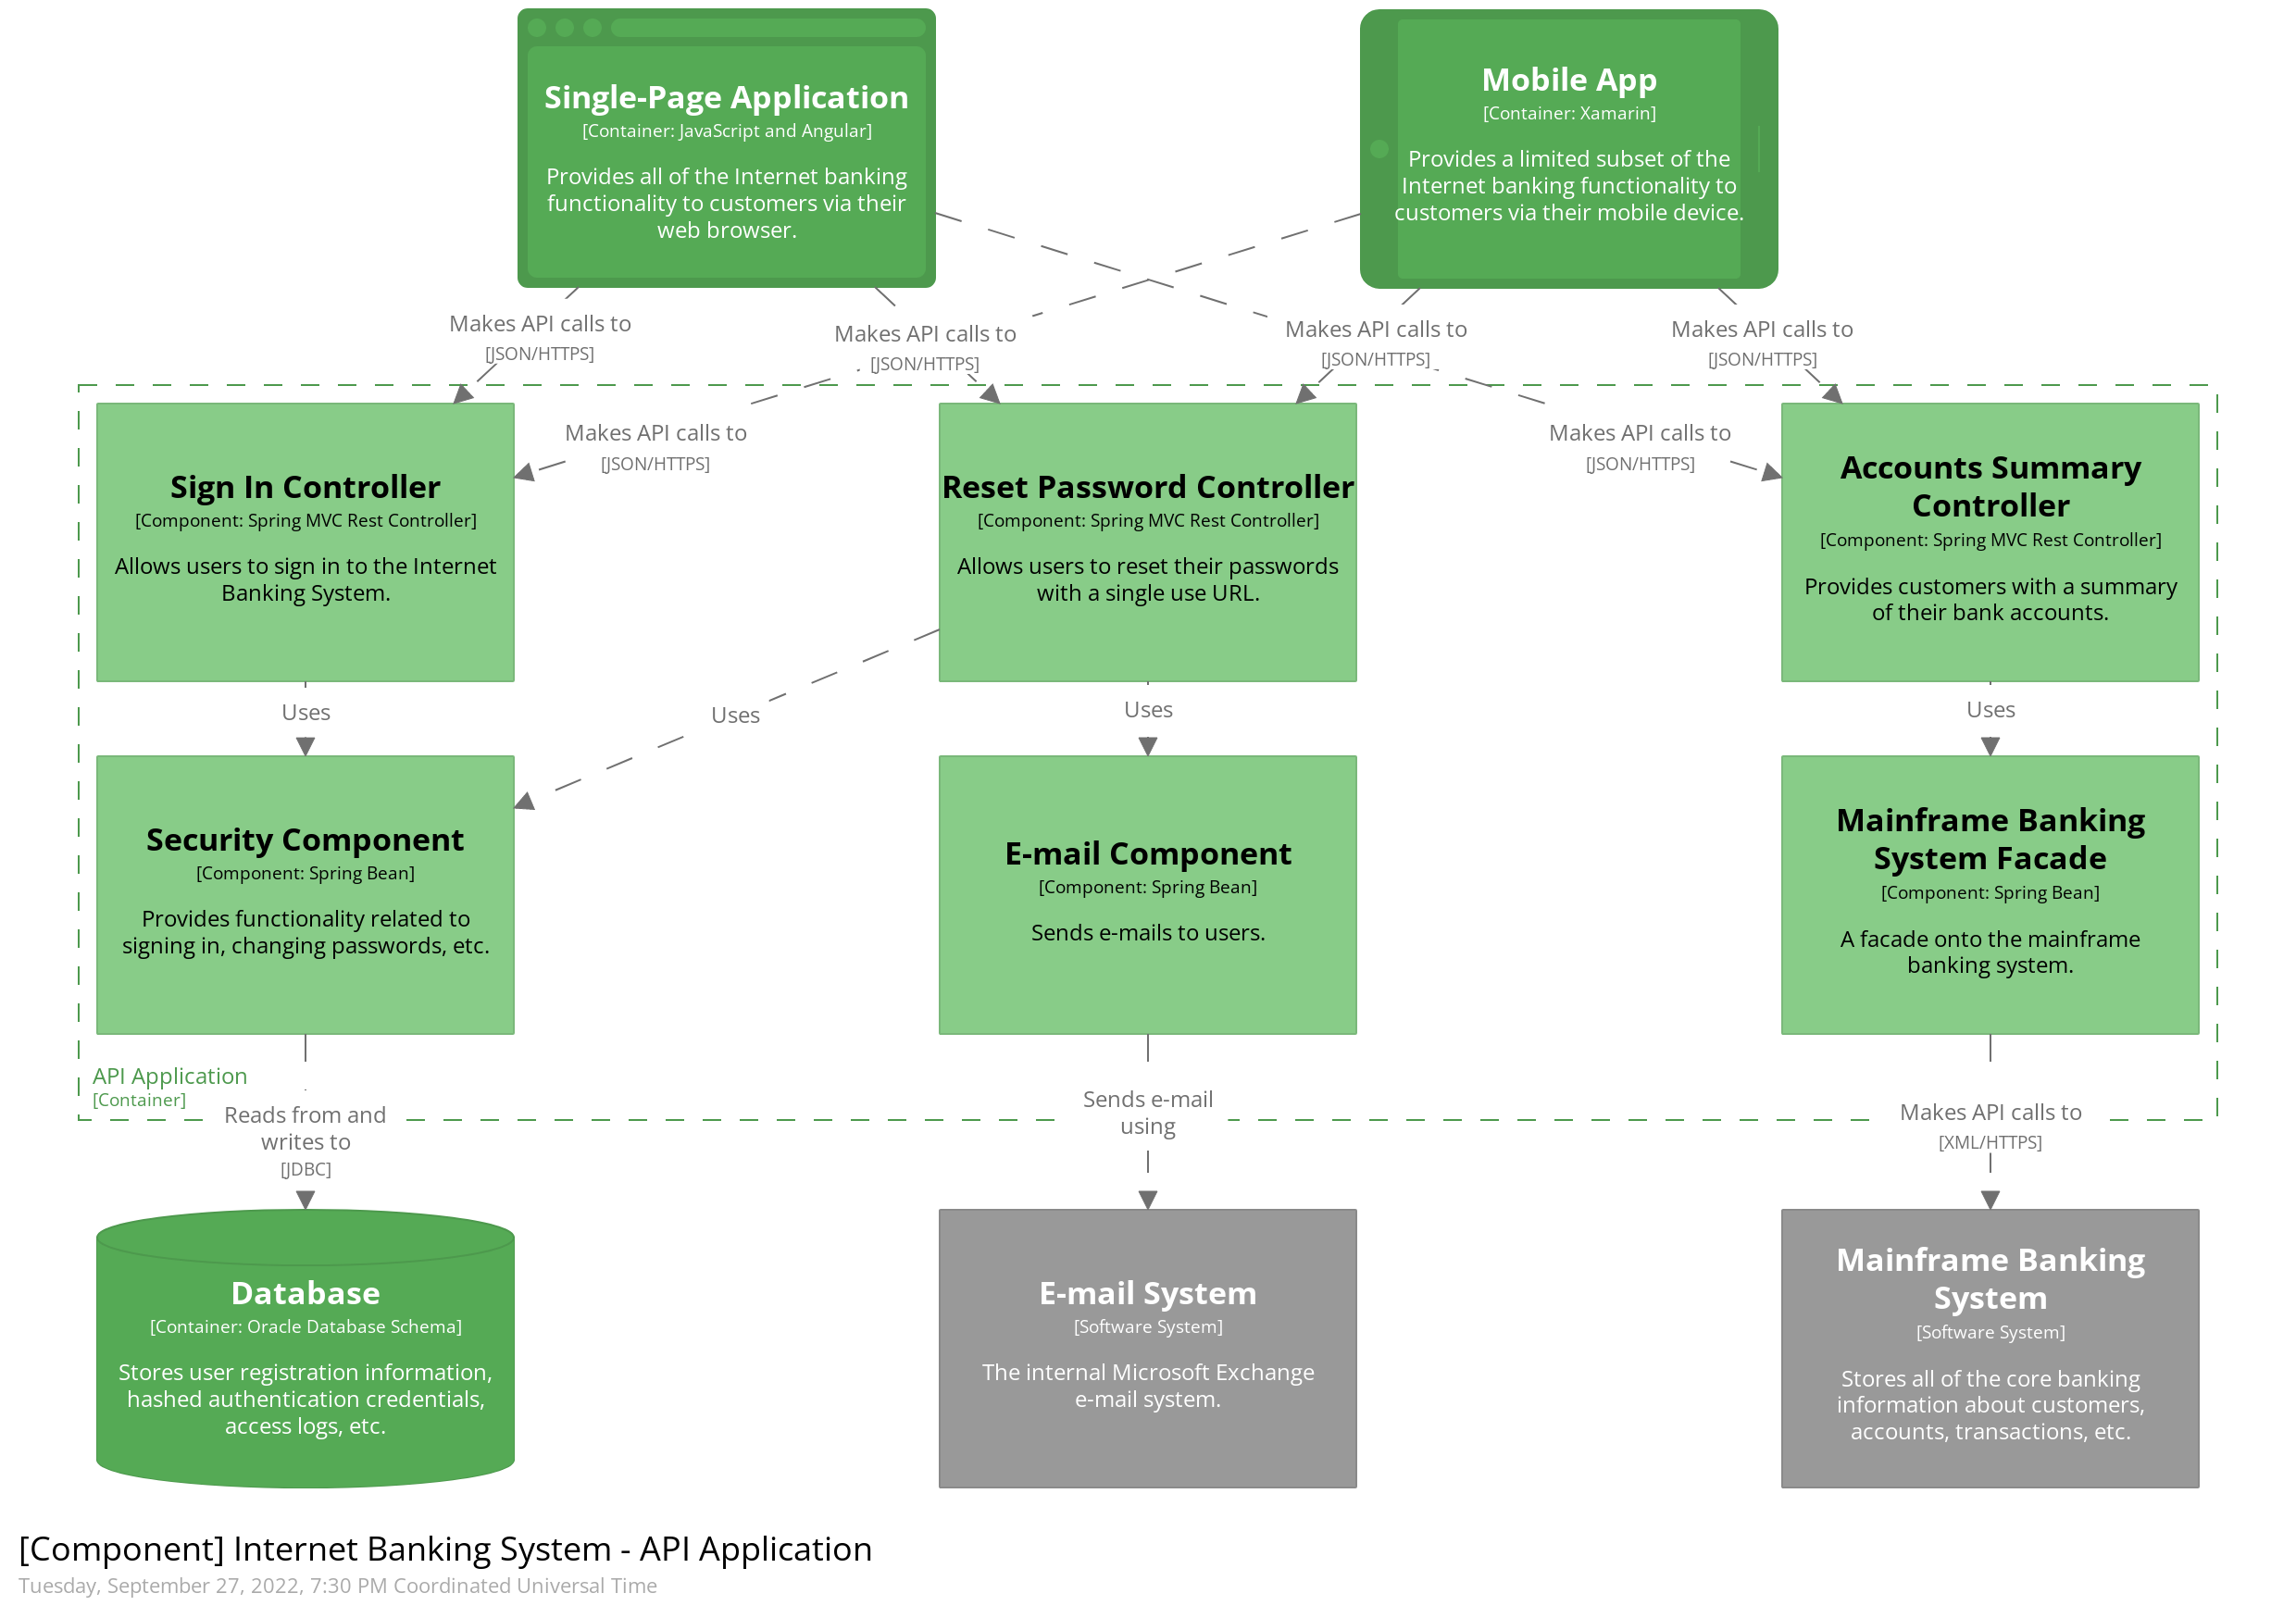
\includegraphics[width=0.75\textwidth]{c4component}
  \caption{C4 Component Diagram}
\end{figure}

\subsection{Level 4: Code}
Finally, if you really want or need to, you can zoom into an individual component to show how that component is implemented. There nearly is never the need to draw a Code diagram, since it gives a very low level idea on how the code is structured.